\chapter{Implementation of RoboMission}
\label{chap:implementation-of-robomission}

TBA

\section{System Architecture}

\begin{itemize}
\item FE, BE (+ clean core) -- REST API
\item environment and dependencies: virtualenv; pip, npm
\item make + django-admin tools
\item (analysis and monitoring; attempt to achieve harmony between CLI and browser apps (dashboards, jupyter notebooks))
\item cron -> scheduled jobs
\item development: git, GH (README, docs, issues, project board?), unit tests
\end{itemize}

\section{Frontend}

\begin{itemize}
\item first prototype: Angular + Bootstrap
\item now: ES6, React, Redux, Material Design
\item infrastructure: webpack (create-react-app)
\item TBA: explain each of these used technologies (briefly)
\item localization (react-intl)
\item asynchronous actions (sagas, possibly show a small snippet (e.g. googleAnalyticsSaga to ilustrate the concept, or even comparision of another approaches to asynchronicity)
\item why the change: more flexible and understandable, easier development and bug fixing; TBA: show how the code is more readable with ES6, how the flow of events is easier to reason about in React+Redux (than in Angular) and how Material Design is more user-friendly than Bootstrap
\item parsing task source, space world, robo code (PEG grammars)
\item Blockly
\item JS-interpreter
\end{itemize}

\section{Backend}

\begin{itemize}
\item Python 3.5, virtualevn, pip
\item Django, Django Rest Framework, (+ many small libraries, such as Django Rest Pandas)
\item django apps (python packages): learn, monitoring
\item models (...), serializers, views, services/use cases/core
\item data export
\item monitoring app, metrics computation
\end{itemize}

\section{Clean Core}

\begin{itemize}
\item TBA: describe the idea, ref relevant book/papers
\item pros/cons
\item Django - possibilities:
\item first attempt -- state, actions, pure reducers -> new state -> diffing; efficiency problems
\item another possible approaches: DB facade ("state", "world", mutable) passed to the services;
  deffered computation (using Django's Q/F values); coroutines to communicate between top-level IO layer and the clean core
\end{itemize}


\section{Server}

\begin{itemize}
\item nginx, gunicorn, git, virtualenv
\item PostgreSQL
\item cron -> scheduled jobs
\end{itemize}


\section{Analysis}

\begin{itemize}
\item (consider) better place for this section
\item pandas, (numpy, matplotlib, sklearn, seaborn)
\end{itemize}


\section{Tasks Description}

\begin{itemize}
\item in markdown (why)
\item online task editor
\item internal represenation (DB model and its serializers for FE and for CSV exports)
\item PEG grammars for whole task source, Space World (ref section below),
  and solution in RoboCode (ref section below)
\end{itemize}

Example of complete task source (for rendered task see figure \ref{fig:robomission-task1}.)

\begin{lstlisting}
# turning-left
- category: moves

## Setting

```
|bM|b |b |bM|b |
|kA|k |kM|k |kA|
|k |k |kA|kM|k |
|kM|k |kS|k |kA|
```

## Solution

```python
left()
fly()
fly()
```
\end{lstlisting}


\section{SpaceWorld Grammar}

\begin{itemize}
\item TBA
\item together with RoboCode allows for a task sources in human-readable and editable markdown (TODO: insert example of space world and also of full task source with rendered game preview), and convenient online task editor
\end{itemize}


\begin{figure}[h]
\begin{center}
\begin{subfigure}{.4\textwidth}
\centering
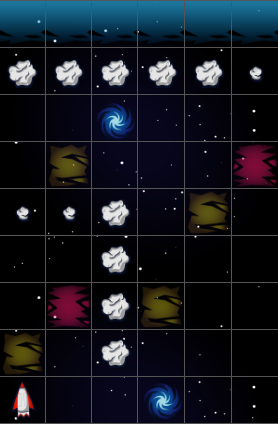
\includegraphics[width=.9\textwidth]{img/spaceworld}
\end{subfigure}
\begin{subfigure}{.36\textwidth}
\centering
{\lstset{numbers=none}
\begin{lstlisting}
|b |b |b |b |b |b |
|kA|kA|kA|kA|kA|kM|
|k |k |kW|k |k |k |
|k |y |k |k |k |r |
|kM|kM|kA|k |y |k |
|k |k |kA|k |k |k |
|k |r |kA|y |k |k |
|y |k |kA|k |k |k |
|kS|k |k |kW|k |k |
\end{lstlisting}}
\end{subfigure}
\end{center}
\caption{Example of Space World with its source code. TODO: Describe letters; consider replacing code listing with a screenshot from task editor with code highlighting}
\label{fig:spaceworld-source}
\end{figure}


\section{RoboCode}

\begin{itemize}
\item new programming language (RoboCode)
\item transformations (ast <-> RoboCode, MiniRoboCode, Blockly, JS)
\item common roboAST representation serves as a mediator between different languages
      that we need to support (Blockly for kids, RoboCode for writing,
      MiniRoboCode for logging, JS for running)
\item (allows for some cool magic such as immediate bidirecitional translating between blockly and RoboCode)
\item describe RoboCode PEG grammar and roboAST, iclude same example rules and parse trees
\item describe miniRoboCode format
\item describe RoboBlockly
\item describe RoboCodeJS
\item describe JS interpreter of RoboCodeJS
\end{itemize}

Example RoboCode, solution of the "Red Shooting" task (currently in figure: \ref{fig:spaceworld-source}), TBA: also include MiniRoboCode, JS, Blockly and AST for complete example.

\begin{lstlisting}
while color() != 'b':
    if color() == 'y':
        right()
    if color() == 'r':
        shoot()
    fly()
\end{lstlisting}
